\documentclass[titlepage,12pt,a4paper]{article}

\usepackage[left=2cm,top=3cm,right=2cm,bottom=3cm,bindingoffset=0.5cm]{geometry}
\usepackage{amsmath}
\usepackage{amssymb}
\usepackage{enumitem}
\usepackage{commath}
\usepackage{mathtools}
\usepackage{graphicx}
%\usepackage{csquotes}
%\usepackage{dirtytalk}
\usepackage{hyperref}
\usepackage{tabto}
\usepackage{gensymb}
\usepackage{graphicx}
\usepackage{listings}
\usepackage{sidecap}
\usepackage{wrapfig}
\usepackage{picinpar}
\usepackage{parskip}
\usepackage{units}
\usepackage{upgreek}
%\usepackage{tabularx}
\usepackage{appendix}

\usepackage{fancyhdr}
\usepackage{color}
\definecolor{dkgreen}{rgb}{0,0.6,0}
\definecolor{gray}{rgb}{0.5,0.5,0.5}
\definecolor{mauve}{rgb}{0.58,0,0.82}

\lstset{frame=tb,
  language=C++,
  aboveskip=3mm,
  belowskip=3mm,
  showstringspaces=false,
  columns=flexible,
  basicstyle={\small\ttfamily},
  numbers=left,
  numberstyle=\footnotesize,
  stepnumber=1,
  numbersep=5pt,
  keywordstyle=\color{blue},
  commentstyle=\color{dkgreen},
  stringstyle=\color{mauve},
  breaklines=true,
  breakatwhitespace=true,
  tabsize=3
}


\pagestyle{fancy}\lhead{A} \rhead{C}
\chead{{\large{\bf B}}}
\lfoot{}
\rfoot{\bf \thepage}
\cfoot{}

\setlength{\headheight}{15.2pt}
\pagestyle{fancy}
\fancyhf{}
\lhead{ \fancyplain{}{COMP3431: Robotic Software Architecture} }
\rfoot{ \fancyplain{}{\thepage} }


\begin{document}
\begin{titlepage}
    \begin{center}
        \vspace*{3cm}
        
        \Huge
        \textbf{COMP3431\\}
        \title{}
        \vspace{0.5cm}
        \Huge
        \textbf{Robotic Software Architecture}
        
        \vspace{0.54cm}
        
        \Large
        Assignment 2: Report
        
        \vspace{5cm}

	\large
	Nathan ADLER \hspace*{10pt} z3327870\\
	Aneita YANG \hspace*{24pt} z5017723\\

	\vfill
        
        \Large
        November 9, 2015
        
    \end{center}
\end{titlepage}

\pagebreak
\tableofcontents

\pagebreak
\section{Introduction}
In this assignment, both the hardware and software aspects of robotics are explored. The overall objective was to create a robot that could navigate autonomously in an outdoor environment, whilst avoiding any obstacles. An existing ground vehicle platform, developed by student society CREATE UNSW, was used as a base for testing.

To achieve the objective, the robot is equipped with a GPS and compass (using an Android phone running ROS). A laser scanner is also attached to the front of the robot, gathering information about the robot's immediate surroundings.

\subsection{Modules}

\subsubsection{Hardware}

The key hardware elements that combine to provide sensory information, networking and control are as follows:

\begin{itemize}
	\item A laptop, to run the ROS core and all nodes that interpret sensory information and output control commands
	\item A LIDAR that provides a 2D field of view of any nearby obstacles
	\item A phone that provides GPS and compass data
	\item A motor controller system and motors that drive the robot
	\item A real-time kinematic (RTK) GPS positioning module that provides centimetre-level accuracy in good conditions
\end{itemize}



\subsubsection{Software}

On the software side, six nodes run in conjunction to operate the robot:

\verb|dest_sender| keeps track of the robot's remaining waypoints.

\verb|gps_drive| calculates and publishes the direction in which the robot needs to travel to reach its destination.

\verb|rtk_gps_pub| publishes an optional precise position based on realtime kinematic GPS solutions with centimetre-level accuracy.

\verb|laser_safe| publishes movement messages, either directly to the bot's destination, or to avoid an obstacle.

\verb|motordata_arduino_send| converts movement messages into serial messages to send to the Arduino that controls the motor driver. This node is what drives the robot.

\verb|sick_tim| reads data from the SICK TiM551 2D laser scanner and publishes the data as a \verb|laser_scan| ROS message.

\pagebreak
\section{Hardware}

\subsection{Mechanical Structure}
The Unmanned Ground Vehicle (UGV) was developed to serve as an autonomous platform for the research and testing of robotic systems. It measures \unit[1]{metre} long, \unit[0.5]{metres} wide and, when fully loaded, weighs approximately \unit[50]{kg}. The robot was constructed using parts from an electric wheelchair and a custom-design welded steel chassis, as shown in Figure \ref{figure:ugv_chassis}.

\begin{figure}[h!]
	\centering
	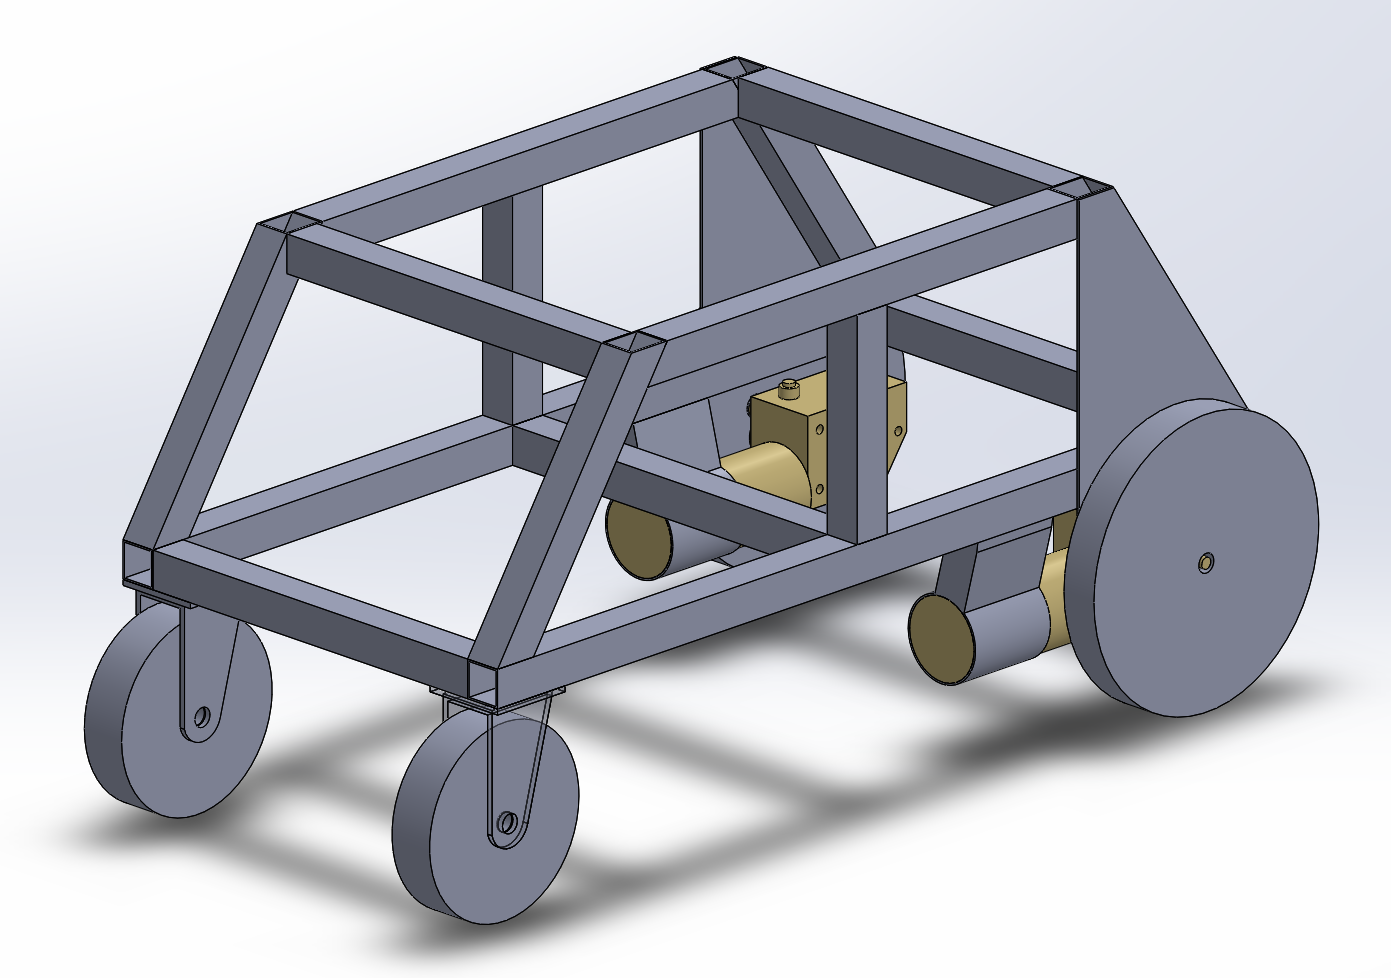
\includegraphics[scale=0.5]{figures/UGV.png}
	\caption{CAD model of chassis of UGV}
	\label{figure:ugv_chassis}
\end{figure}

\subsection{Specifications and Drivers}
\subsubsection{SICK TiM551 2D Laser Scanner}


%\begin{table}[h!]
%	\caption{SICK TiM551 Specifications}
%	\label{table:spec}
%	\begin{tabular}{|c|c|}
%		\hline
%		Aperture angle & \unit[270]{\degree}\\
%		Scanning frequency & \unit[15]{Hz}\\
%		Angular resolution & \unit[1]{\degree}\\
%		Operating range & \unit[0.05-10]{m}\\
%		\hline
%	\end{tabular}
%\end{table}


The 2D laser scanner (shown in \figref{figure:sick_lidar}) is rated outdoor IP67, allowing for use in a variety of weather conditions including bright sunlight. The sensor provides readings up to a maximum range of \unit[10]{m}, giving enough perspective to traverse routes in terrain with complex and even dynamic obstacles. The following specifications detail the capabilities of the sensor: 

\begin{itemize}
	\item Aperture angle: \unit[270]{\degree}
	\item Scanning frequency: \unit[15]{Hz}
	\item Angular resolution: \unit[1]{\degree}
	\item Operating range: \unit[0.05-10]{m}
	\item Operating voltage: \unit[9-28]{V} DC
	\item Power consumption: \unit[3]{W}
\end{itemize}

\begin{figure}[h!]
	\centering
	
	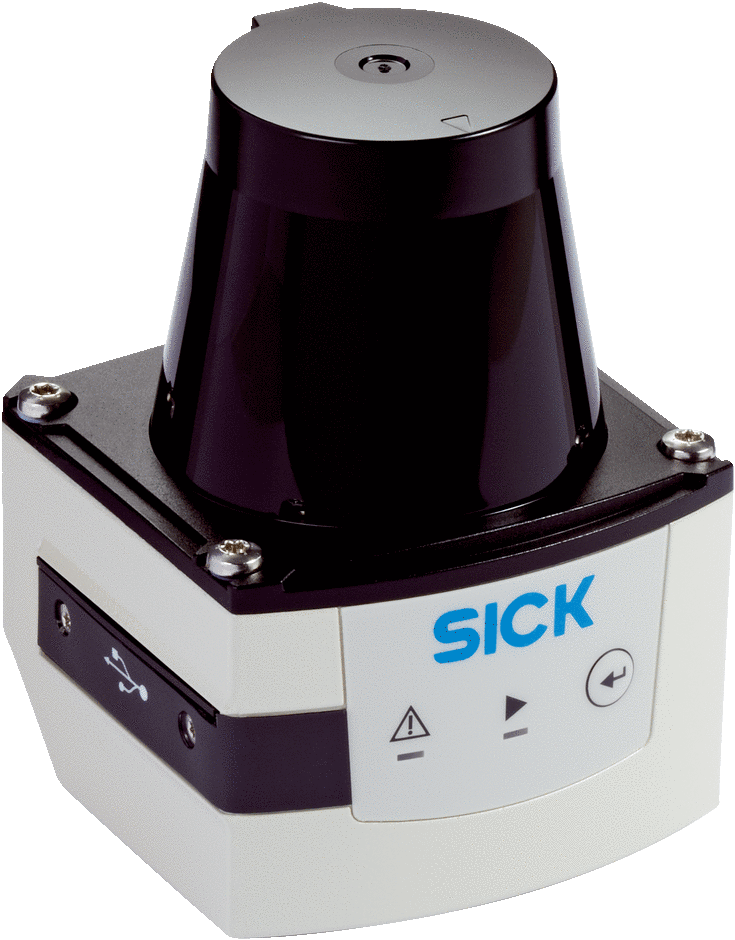
\includegraphics[scale=0.2]{figures/sick_lidar.png}
	\caption{\textbf{SICK TiM551 2D Laser Scanner}}
	\label{figure:sick_lidar}
\end{figure}

The device is mounted in a static location on the front of the UGV in the horizontal plane approximately \unit[300]{mm} above ground level. In this position, the view is partially obscured to the sides and behind the laser scanner by the UGV chassis and, therefore, the view is limited to a \unit[150]{\degree} sweep to the front of the robot in software.

To obtain data from the laser scanner, the open source \verb|sick_tim| ROS package is used. The package provides a launch file \verb|sick_tim551_2050001.launch|, which reads range data into a \verb|sensor_msgs/LaserScan.msg| that is published every scan frame.

\subsubsection{Android phone GPS and compass}

The robot is equipped with an Android phone running the \verb|android_sensors_driver| application called ROS All Sensors. The app publishes:

\begin{itemize}
	\item Camera images: \verb|sensor_msgs/CompressedImage| and \verb|sensor_msgs/Image|
	\item Fluid pressure data: \verb|sensor_msgs/FluidPressure|
	\item Illuminance data: \verb|sensor_msgs/Illuminance|
	\item Accelerometer: \verb|sensor_msgs/Imu|
	\item Magnetic field: \verb|sensor_msgs/MagneticField|
	\item GPS fixes: \verb|sensor_msgs/NavSatFix|
	\item Temperature data: \verb|sensor_msgs/Temperature| \\
\end{itemize}

During operation, camera streaming is not enabled to ensure there is enough bandwidth and processing available for proper operation of all software modules. The GPS receiver is able to use American GPS and Russian GLONASS satellites, and provides a ``fix" solution at a rate of \unit[1]{Hz}. The fix solution is formatted as a \verb|sensor_msgs/NavSatFix.msg| (see \appref{appendix:NavSatFix.msg}) All other sensor data is published at a rate of \unit[20]{Hz}.

\subsubsection{RTK GPS Module}

A specialised GPS device (shown in \figref{figure:RTK_GPS_device}) is mounted on the UGV for precise positioning. It consists of an antenna with an inbuilt raw receiver, and an Odroid U3 with a 3G dongle. The open source software computes centimetre-accurate positions at \unit[2]{Hz} and is configured to output solutions over TCP connection through the VPN. The latitude and longitude solutions are then received and published as a \verb|NavSatFix.msg| by \verb|rtk_gps_pub|.

\begin{figure}[h]
	\centering
	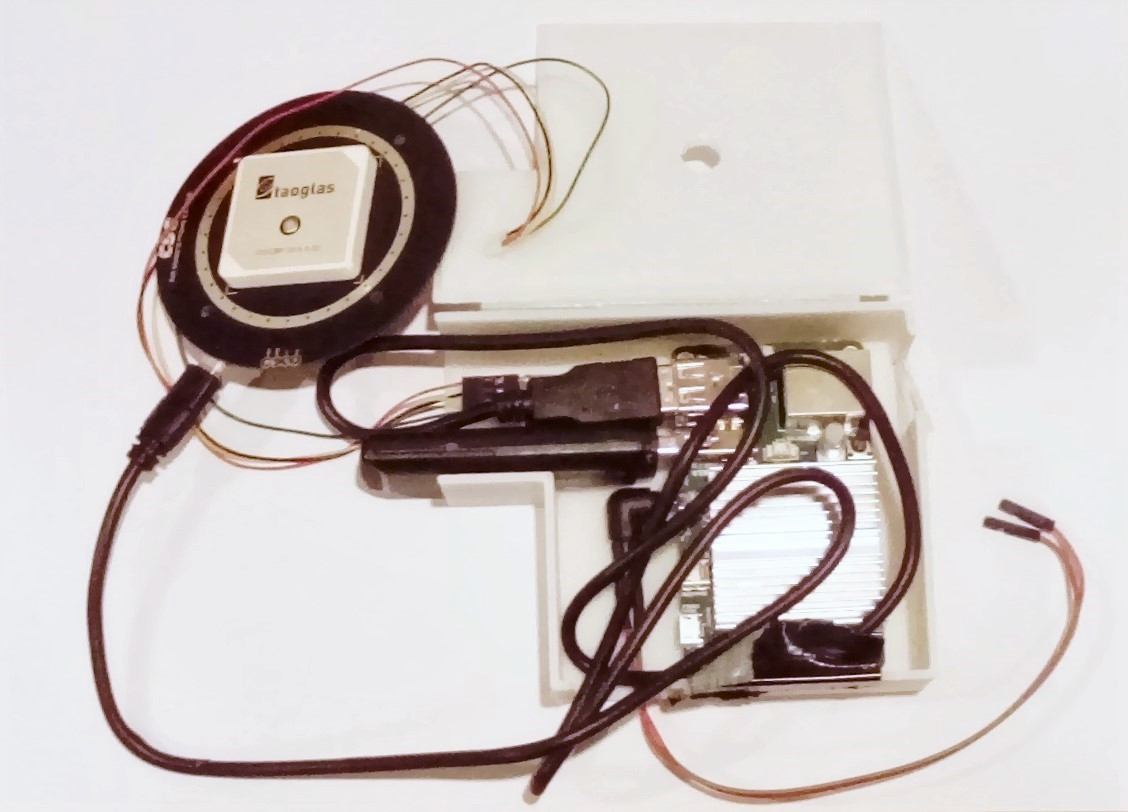
\includegraphics[scale=0.2]{figures/rtk_gps.jpg}
	\caption{\textbf{RTK GPS precise positioning device mounted on UGV}}
	\label{figure:RTK_GPS_device}
\end{figure}

\subsubsection{Arduino and Motor Driver}
\label{motor_driver_explanation}

The dual-channel motor driver converts a pulsed signal to pulse-width modulated (PWM) output to drive the motors in either direction. The pulse ranges from control ranges from \unit[1000-2000]{$\upmu$s}, where 1500 is off, 2000 is full forward and 1000 is full reverse. The pulse signals are generated by the Arduino Mega 2560 microcontroller, which is connected to the laptop via USB.. The microcontroller is programmed to receive messages in a custom format as follows:

\begin{center}
	[SAADBB:CC]
\end{center}

where S is direction of bridge A, either '+' or '-', AA is the PWM of bridge A, from 00 to FF, D is direction of bridge B, either '+' or '-', BB is the PWM of bridge B, also from 00 to FF, and CC is the checksum of the command. The Arduino then scales and converts the command into the appropriate pulse signal timing to output to the dual-channel motor driver.

The Arduino program also includes motor controls that smooth changes in speed and direction to avoid damaging the motors, and a watchdog timer that stops the motors if no new command has been received for \unit[500]{ms}.


\pagebreak


\subsection{Integration}

The following hardware is contained on board:

\begin{itemize}
	\item Dell Latitude E6400 notebook
	\item SICK TiM551 2D laser scanner
	\item DLink DSL 2750B N300 Modem Router
	\item Sony Xperia Z3 compact
	\item Arduino Mega 2560 R3
	\item Sabertooth 2X25 regenerative motor driver
	\item 2 x 12V lead acid battery
	\item 2 x electric wheelchair motor
\end{itemize}

\begin{figure}[h!]
	\centering
	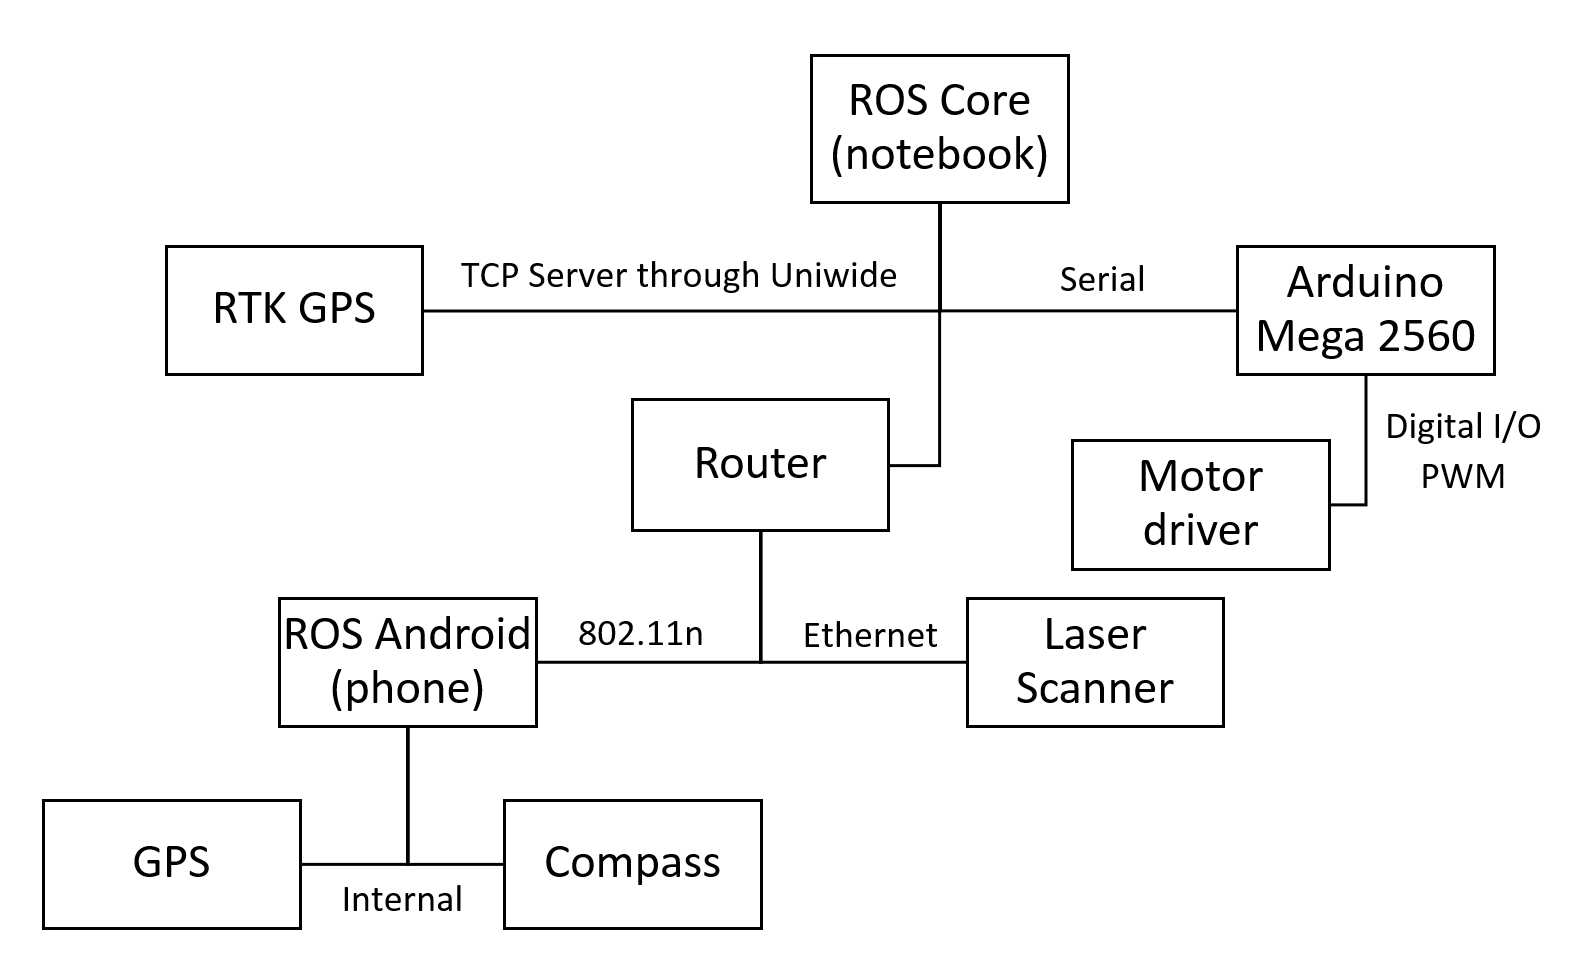
\includegraphics[scale=0.6]{figures/hardware_chart.png}
	\caption{\textbf{Hardware map of UGV}}
	\label{figure:hardware_chart}
\end{figure}

The Dell notebook is installed with Ubuntu 14.04 (a.k.a. "Trusty Tahr") and ROS Indigo. Sensors from the phone and laser scanner are integrated in a Local Area Network through a combination of Ethernet and wireless connections. A VPN is installed for remote communication over the internet between networked devices, including a precise positioning GPS device developed for an undergraduate thesis. \unit[24]{V} power from the two lead acid batteries is supplied to the motor driver to power the DC geared motors and integrated solenoid brakes. \unit[12]{V} from one of the batteries is segmented to provide a separate power source for the laser scanner and the router.

\textbf{Note:} this hardware configuration was not set up prior to undertaking this assignment (excluding the chassis, motors and motor driver); all hardware development and integration was conducted as part of the project.

\pagebreak
\section{Software}

Three main modules run in conjunction to govern the UGV: planner, localisation and waypoint traversal.

\begin{figure}[h]
	\centering
	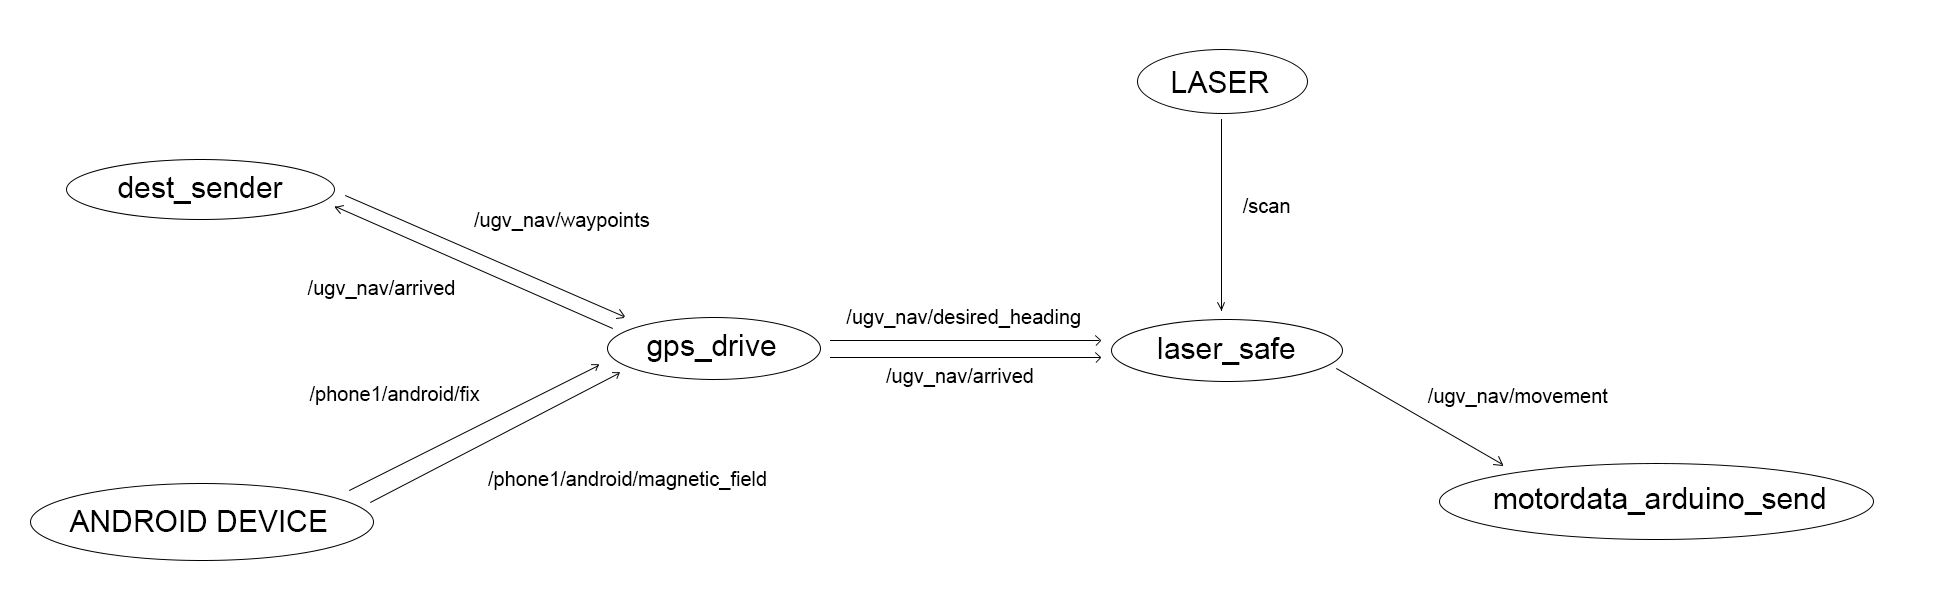
\includegraphics[scale=0.255]{figures/rqt.png}
	\caption{\textbf{Rqt graph.}}
\end{figure}

\subsection{Planner}
The planner module is responsible for keeping track of the robot's waypoints and informs the robot of its next destination. 

The \verb|dest_sender| node parses a file containing the GPS coordinates of waypoints and turns each latitude-longitude pair into a NavSatFix message. Each waypoint is stored in a list (as a NavSatFix message), with the head of the list being the robot's next destination. \verb|dest_sender| publishes this message to the \verb|/ugv_nav/waypoints| topic for other modules to subscribe to.

\verb|dest_sender| subscribes to the \verb|/ugv_nav/arrived| topic, which signals when the robot has reached its destination. Messages which are published to the \verb|/ugv_nav/arrived| topic trigger a callback which removes the current waypoint from the list (i.e. the head of the list). If the robot has not reached its final destination and the list is not empty, the robot's next destination is published.

\subsection{Localisation}

\subsubsection{UGV position and heading determination}
The localisation module is responsible for determining the direction in which the robot needs to travel to reach its goal. In order to determine this direction, the robot must be aware of its position in GPS coordinates, its bearing from true north and the GPS coordinates of its destination.

For this assignment, the \verb|gps_drive| node performs these required calculations. In particular, the \verb|gps_drive| node subscribes to the Android device's GPS fixes and magnetic fields (published on the \verb|/phone1/android/fix| and \verb|/phone1/android/magnetic_field| topics respectively). The robot also has the option to receive real-time kinematic GPS data through \verb|/ugv_nav/rtk_fix|, providing a more accurate position from an external GPS module in good conditions. A filter is implemented that determines whether the RTK GPS data is suitable for use by ensuring that the five latest readings (2.5 seconds of data) are within an acceptable area. If the RTK GPS does not have a good fix solution, the positioning calculations revert to using the phone GPS.

The GPS coordinates of the robot's destination are published to the  \verb|/ugv_nav/waypoints| topic by the \verb|dest_sender| node, which \verb|gps_drive| also subscribes to.

\subsubsection{Waypoint bearing calculation}
\begin{figure}[h]
	\centering
	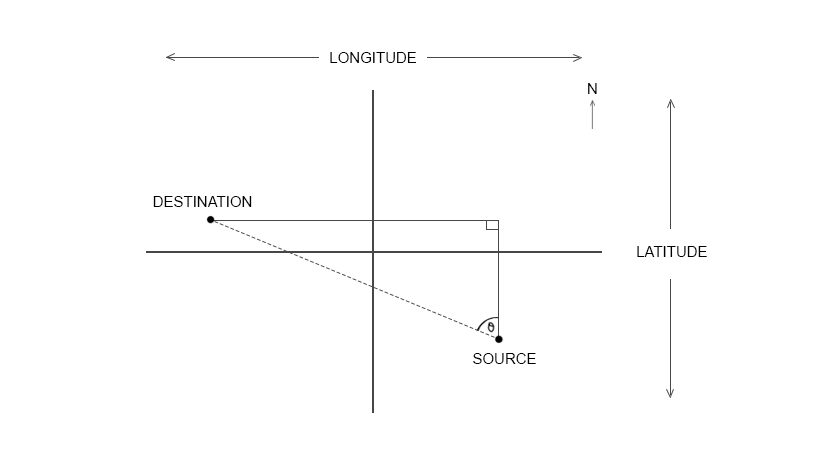
\includegraphics[scale=0.6]{figures/bearings.png}
	\caption{\textbf{Calculation of the bearing of the destination from the robot, if the robot is facing true north.}}
	\label{figure:bearing1}
\end{figure}

Calculating the bearing of the destination from the robot is dependent on the GPS coordinates of both the robot and the destination.
\begin{equation}
	\begin{split}
		\Delta{latitude} = \text{destination\_latitude - robot\_latitude}\\
		\Delta{longitude} = \text{destination\_longitude - robot\_longitude}\\
	\end{split}
\end{equation}

Supposing the robot is facing True North, and if $\beta$ is the bearing of the destination from the robot then:
\begin{equation}
	\beta = \tan^{-1}({\frac{\Delta{longitude}}{\Delta{latitude}}})
\end{equation}
If $\theta$ is the angle the robot must turn to reach its destination, as in Figure \ref{figure:bearing1}, then $\theta = \beta$.

In the cases where the robot is not facing true north, then:
\begin{equation}
	\theta =	(-\alpha) + \beta
	\label{equation:desired_heading}
\end{equation}
where:
\begin{equation}
\begin{split}
	\beta =	\tan^{-1}({\frac{\Delta{longitude}}{\Delta{latitude}}})\\
	\alpha = \tan^{-1}(\frac{x}{y})
\end{split}
\end{equation}
where $x$ and $y$ are magnetic field strength to the top and right edges of the mobile phone respectively.

\begin{figure}[h]
	\centering
	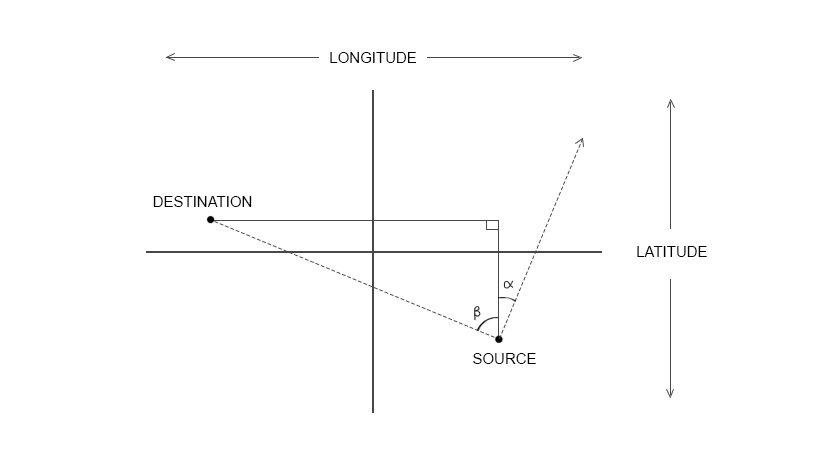
\includegraphics[scale=0.6]{figures/bearingsOffset.png}
	\caption{\textbf{Calculation of the bearing of the destination from the robot where the robot is not facing true north. NOTE: In this example, $\alpha$ is positive and $\beta$ is negative.}}
\end{figure}

\pagebreak

\text{Since at the latitude of Sydney, one degree of latitude is approximately \unit[111]{km}:}

\begin{equation}
	\text{distance\_to\_destination} = 111000 \cdot \sqrt{\text{difference\_lat}^2+ \text{difference\_long}^2}
\end{equation}

If the distance to the destination is less than 5 (i.e. the robot is within 5 metres of its destination), it is considered to have arrived at its destination. At this stage, the \verb|gps_drive| node will publish a message to the \verb|/ugv_nav/arrived| topic, signalling to the \verb|dest_sender| that the robot has reached its destination and that a new destination is required.

Because of the inaccuracies of the compass and the GPS, the vehicle may have a tendency to deviate from the straight line path between waypoints. This can result in the robot wandering off the most suitable path. To counter this, a bias toward the straight line path is added to direct the robot back on track. The bias is made proportional to the perpendicular distance from the straight line path according to the following equation:

\begin{equation}
bias = k * \text{distance\_to\_destination} * sin(\text{desired\_heading}-\text{start\_to\_dest\_heading})
\end{equation}

where \(k\) is the proportional constant, chosen to be 2, and \verb|start_to_dest_heading| is the heading from either the starting position or the last waypoint to the current destination. For example, if the position is calculated to have deviated \unit[5]{m} from the straight line path, then the robot will adjust its bearing \unit[10]{\degree} in addition to the new straight line bearing.


Following these calculations, the \verb|gps_drive| node publishes the most applicable bearing (as a std\_msgs::Float32 message) for the robot to travel. The waypoint traversal module then performs the applicable actions based on this bearing.


\subsection{Waypoint Traversal}
The waypoint traversal module is responsible for physically getting the robot to its destination. The \verb|gps_drive|, \verb|laser_safe| and \verb|motordata_arduino_send| nodes work in conjunction to achieve this goal.

\subsubsection{Obstacle Avoidance}
To detect any obstacles in the robot's path, a laser scanner is attached to the front of the robot.

Given a bearing to travel along, the \verb|laser_safe| node will take one of two courses of action. If there is no obstacle in front of the robot, the robot will drive in the direction it was instructed to by the \verb|gps_drive| node. If an obstacle is present, however, the robot's first priority is to avoid colliding with the obstacle. 

\begin{figure}[h]
	\centering
	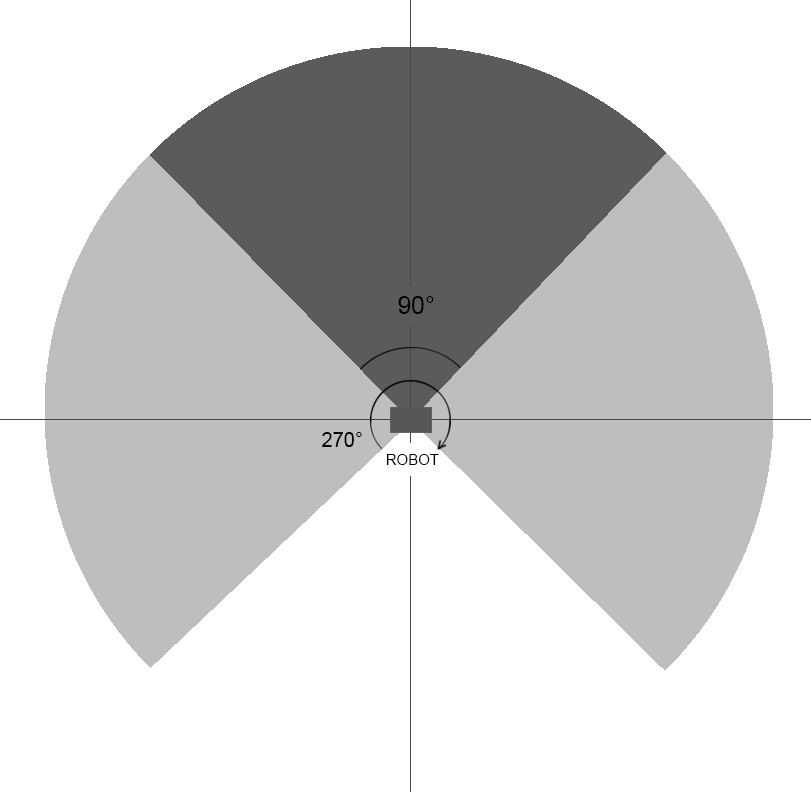
\includegraphics[scale=0.34]{figures/laser.png}
	\caption{\textbf{Range of laser scanner for Iterations 1 and 2.}}
\end{figure}

Note that for the purposes of this assignment, the robot is instructed to scan for obstacles within a \unit[150]{\degree} field-of-view. That is, obstacles further than \unit[75]{\degree} to the left or right of the centre of the robot are deemed as harmless and are ignored.

\textbf{First Iteration}

The first iteration of obstacle avoidance involves bringing the robot to a complete stop when an obstacle enters the view of the laser scanner. As the UGV's main task is to drive autonomously in outdoor environments, this method proves useful for moving obstacles (e.g. people) that may enter and exit the frame quickly. \\

\textbf{Second Iteration}

\begin{figure}[h]
	\centering
	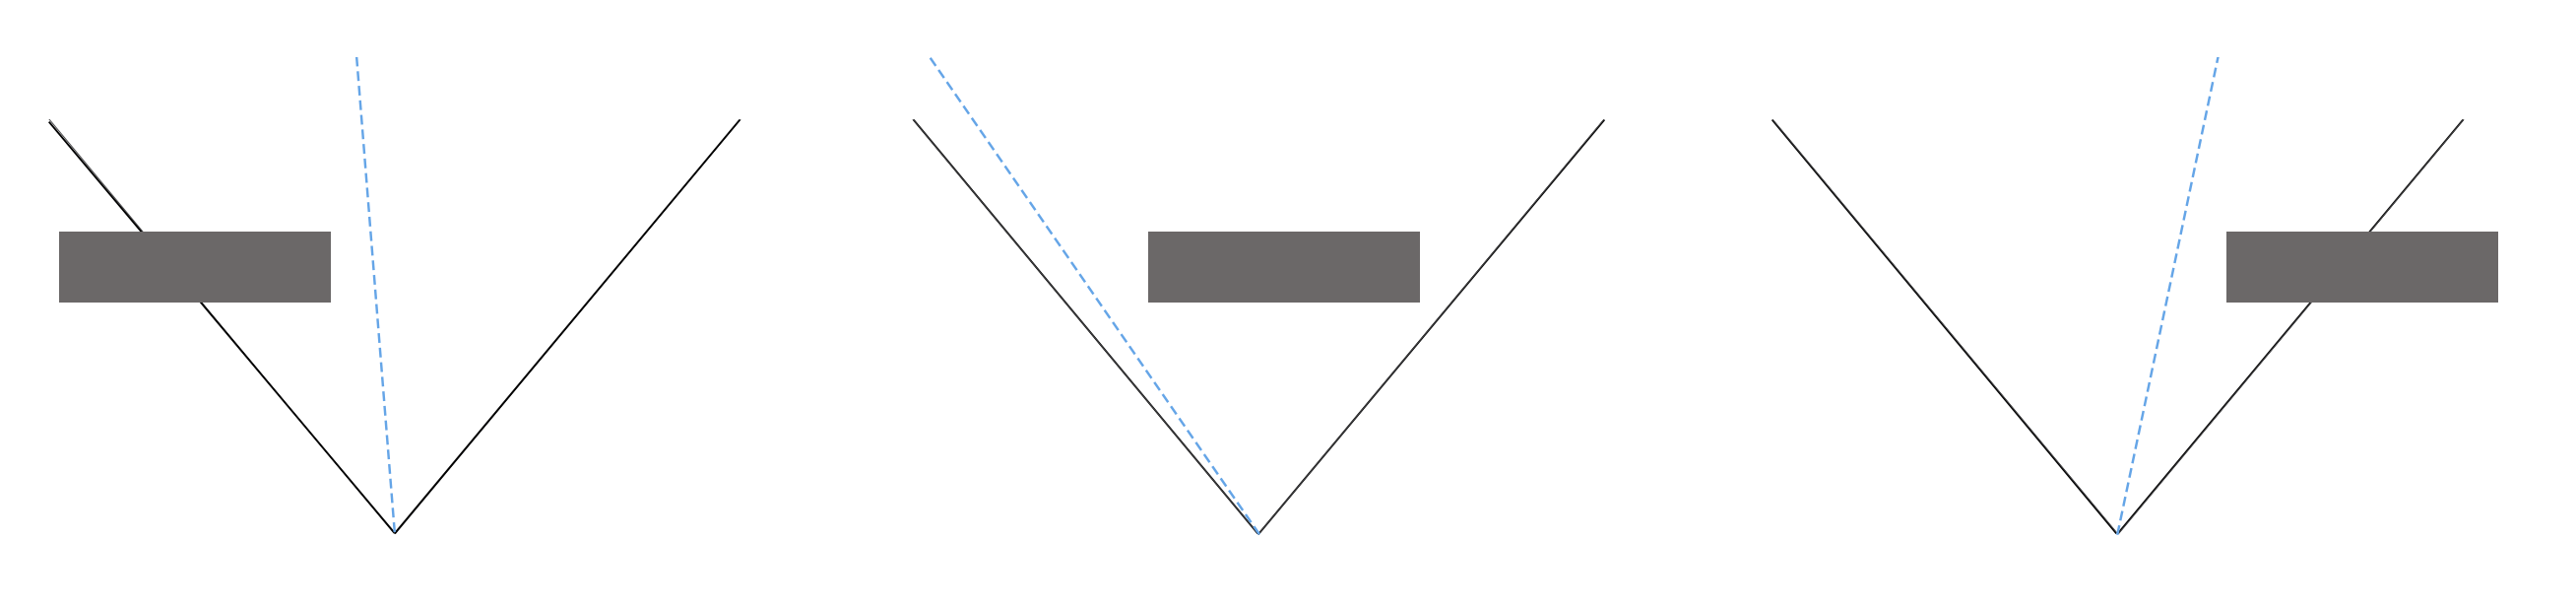
\includegraphics[scale=0.17]{figures/obstacle2.png}
	\caption{\textbf{Obstacle avoidance paths for Iteration 2.}}
\end{figure}

The second iteration of obstacle avoidance attempts to drive around obstacles as they enter the danger zone (i.e. 45\degree left and right of the centre of the robot, within \unit[2]{m}). The robot does this by picking the closest `safe' spot to the left of the first obstacle, if possible, and drives towards it. In cases where the obstacle cuts out of the left-hand side of the laser's frame, the closest `safe' spot to the right is chosen. 

Once the robot is clear of all obstacles, it resumes driving towards its destination. \\


\textbf{Final Iteration}

To handle cases where multiple distinct obstacles are visible, the distance of obstacles needs to be taken into account. The previous obstacle avoidance method is improved by finding the best available heading that is passable, and the width of the robot provides a safe bearing for the robot to travel. The algorithm undergoes the following steps:

\begin{enumerate}
	\item Populate an array the length of the number of ranges in the scan range with '1' for visible obstacles within \unit[3]{m} and '0' for clear space
	\item Widen the bearing occupied by any visible obstacles within the array according to their distance away from the robot, so that a bearing buffer equivalent of \unit[0.7]{m} on either side of the detected obstacle is occupied, using the formula in \eqref{equation:bearing_buffer}.
	\item Choose the available bearing that is closest to the desired bearing calculated in \eqref{equation:desired_heading}. If no bearing is available, do not publish any command for movement.
\end{enumerate}

This process is shown in \figref{figure:obstacle_avoidance_final}. Code for the algorithm can be found in \appref{appendix:obstacle_avoidance}.

Additionally, if any obstacle comes within \unit[0.7]{m} of the robot, a safety stop is enacted and the robot will not move.

\begin{equation}
\begin{split}
	\text{angle\_buffer} = sin^{-1}(\frac{\text{SAFE\_DISTANCE}}{range})\\
	\text{where } \text{SAFE\_DISTANCE} = 0.7
\end{split}
	\label{equation:bearing_buffer}
\end{equation}

\begin{figure}[h]
	\centering
	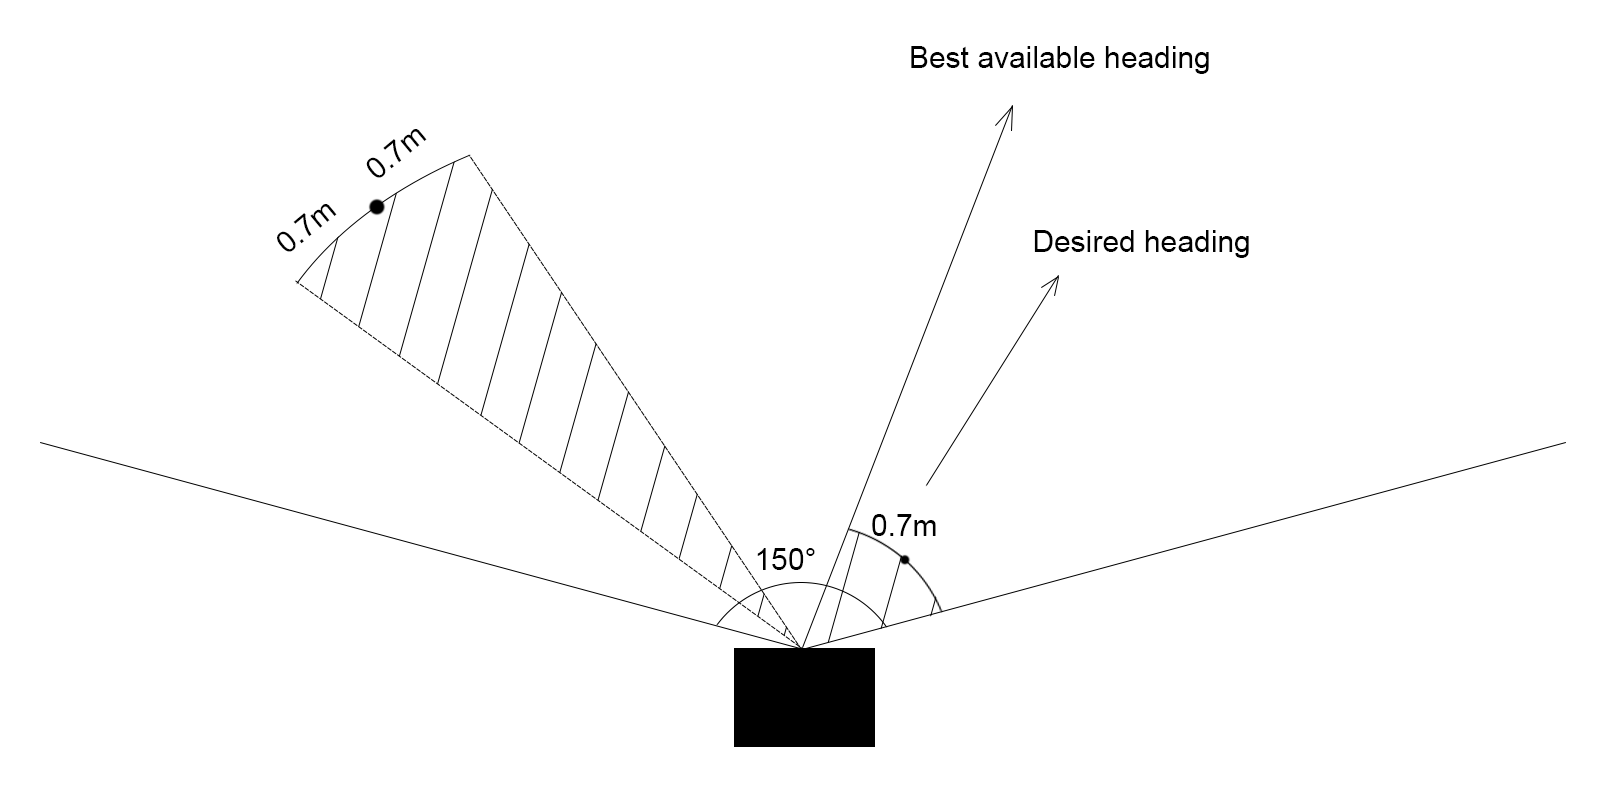
\includegraphics[scale=0.25]{figures/finalObstacle.png}
	\caption{\textbf{Obstacle avoidance for Final Iteration.}}
	\label{figure:obstacle_avoidance_final}
\end{figure}

\subsubsection{Motor Control}

To convert a motion heading into motor commands, a motor behaviour transform is enacted to mimic joystick control for a differentially steered vehicle, such as an electric wheelchair. The function responsible for carrying out this transformation is recorded in \appref{appendix:motor_controller}. The variation of motor power with respect to heading is mapped in \figref{figure:motor_control}.

\begin{figure}[h]
	\centering
	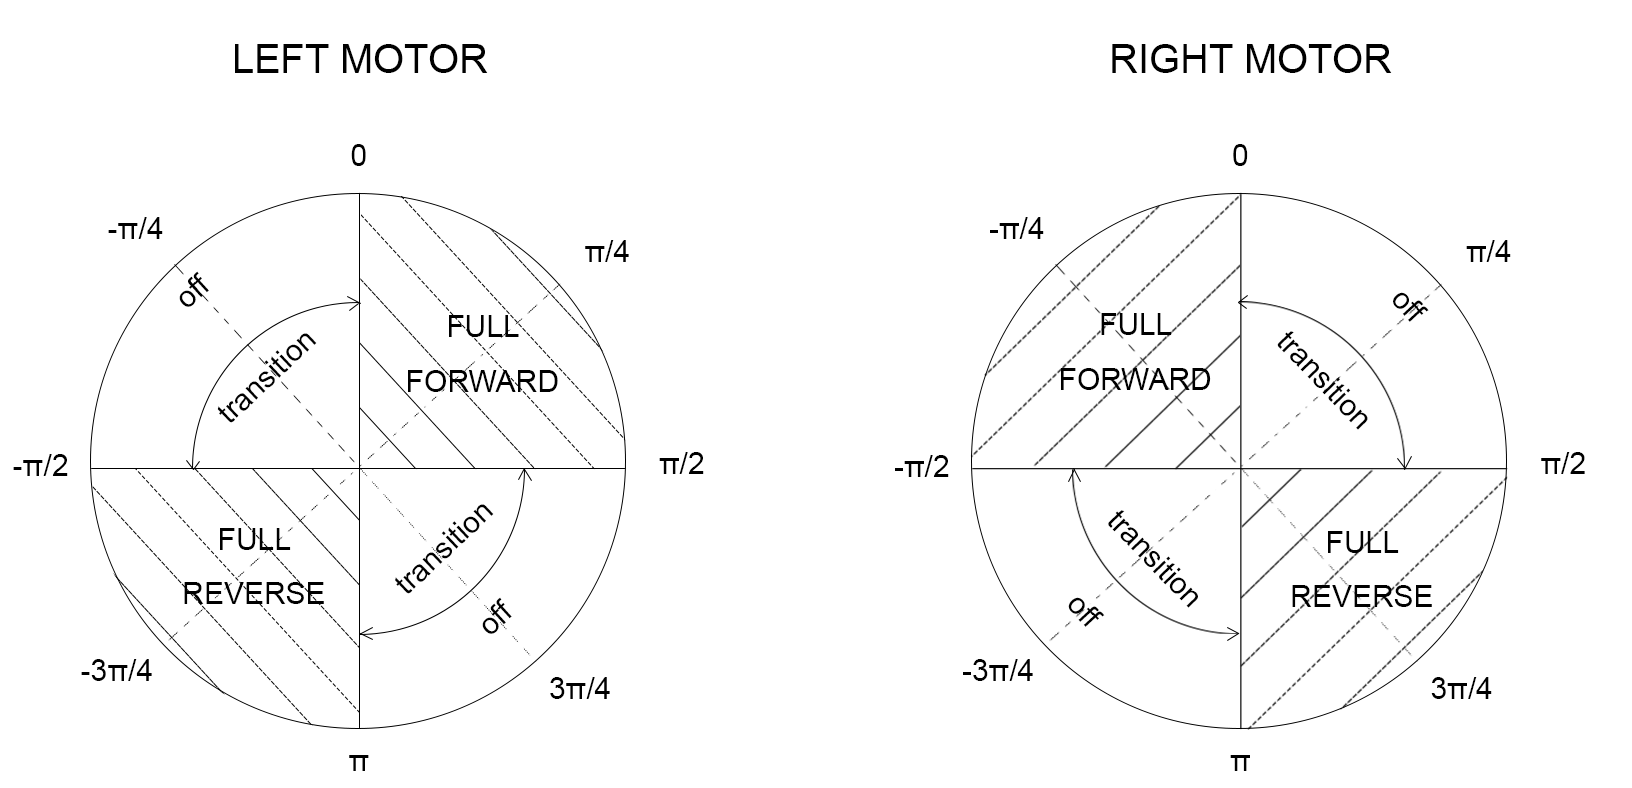
\includegraphics[scale=0.25]{figures/motors.png}
	\caption{\textbf{Motor controls.}}
	\label{figure:motor_control}
\end{figure}

To direct the robot in the direction of the next waypoint according to the calculated heading dependent on bias corrections and obstacle avoidance, a proportional controller is implemented for steering. The local desired heading $\theta$ is halved and then constrained to $\pm$\unit[30]{\degree} to ensure a controlled turn regardless of the difference between the current and desired heading. This guarantees the robot does not drive backwards or carry out a sharp pivot which would risk the robot crashing into obstacles it cannot see. At the same time, the proportional controller allows for subtle changes in direction through varying power to the motors that differentially steer the robot. As the current location and desired heading of the robot are updated at regular intervals, the steering heading of the robot will gradually adjust accordingly.

For testing, the magnitude of the speed control was fixed at 70\%. When traversing between waypoints, if a valid heading was available (no obstacles within \unit[0.7]{m}, no impassable barriers) then a motion command is published. This motion command is updated at \unit[10]{Hz}. The command was formatted according to the requirements of the Arduino motor driver bridge (see \ref{motor_driver_explanation}) and sent over serial.

\pagebreak
\section{Results}

For testing, the \verb|gps_config| file was loaded with a series of 10 waypoint coordinates starting on the lower campus main walkway of UNSW outside the Tyree Energy Technologies building, finishing at the bottom of the Scientia building. The robot then was allowed to drive autonomously as it attempted to complete the journey between the two points. The robot successfully navigated to its destination and then returned, although required some assistance in certain situations.

The demonstration for the assignment performed well in large open areas with no tall surrounding objects. The main causes for incorrect behaviour were poor GPS fixes, blind spots in the laser scanner and interference with the laser scanner. \\

\textbf{Inaccurate GPS Fixes}

Waypoint traversal relies heavily on the robot being able to pinpoint its precise position. In sheltered areas, or areas with tall buildings or trees, GPS fixes can be inaccurate. Such inaccuracies impact on the accuracy of the calculations performed. The bearing of the destination from the robot's position can be incorrect. The distance the robot must drive before reaching its destination can also be wrong. When working with unmanned vehicles, it is particularly important that these calculations are precise and accurate. In circumstances where the robot had a precise RTK GPS fix solution, mainly in areas not in proximity to tall buildings on multiple sides, the driving of the robot was significantly improved.\\

\textbf{Laser Scanner Blind Spots}

The laser scanner is positioned on the front of the robot, on its base. Sitting at a height of \unit[30]{cm} above the ground, the laser scanner scans on a level plane. Obstacles shorter than \unit[30]{cm}, that lie outside of the laser's view, are essentially driven over or driven through. During the demonstration, the robot drove into a brick wall which was just below the laser scanner's view. The robot was also sometimes confused when variations in the gradient of the ground saw it to believe that obstacles were nearby, such as on grassed areas where the laser scanner would detect the grass. The laser scanner's limited view also meant that care had to be taken when the robot was undergoing sharp turns, and this limited its range of motion.\\

\textbf{Laser Scanner Interference}

Obstacle avoidance relies entirely on data received from the laser scanner. In areas with reflective surfaces (e.g. mirrors and glass), the reflection interferes with the laser, causing the robot to think there are obstacles even when the path is clear. This caused the robot to think that certain paths were blocked and try to go around non-existent obstacles. A fix was attempted that involved filtering out detected obstacles the size of only one point, which somewhat improved navigation.

\pagebreak
\section{Future Work and Improvements}

A number of improvements are possible in future revisions of the software on the UGV to enhance navigation capabilities and increase its potential as a platform for research and development. These include:

\begin{itemize}
	\item Adding a depth sensor on front such as Kinect to sense ledges and different terrain.
	\item Adding odometry to better track the movement of the robot.
	\item Implementing an EKF with the odometry to improve errors in positioning.
	\item Adding a sensor on the rear to allow for autonomous reversing.
	\item Implementing map-based localisation and navigation for better path planning.
	\item Extending navigation into indoor environments and manage transition between outdoor and indoor settings.
\end{itemize}

\pagebreak
{\huge \textbf{Appendix}}
\appendix
\addappheadtotoc
\section{sensor\_msgs/NavSatFix.msg}
\label{appendix:NavSatFix.msg}
\begin{lstlisting}[language=C++]
Header header

/* Satellite fix status information */
NavSatStatus status

/* Latitude [degrees]. Positive is north of equator; negative is south. */
float64 latitude

/* Longitude [degrees]. Positive is east of prime meridian; negative is west. */
float64 longitude

/*
Altitude [m]. Positive is above the WGS 84 ellipsoid
(quiet NaN if no altitude is available).
*/
float64 altitude

/*
Position covariance [m^2] defined relative to a tangential plane
through the reported position. The components are East, North, and
Up (ENU), in row-major order.
Beware: this coordinate system exhibits singularities at the poles.
*/
float64[9] position_covariance

/*
If the covariance of the fix is known, fill it in completely. If the
GPS receiver provides the variance of each measurement, put them
along the diagonal. If only Dilution of Precision is available,
estimate an approximate covariance from that.
*/
uint8 COVARIANCE_TYPE_UNKNOWN = 0
uint8 COVARIANCE_TYPE_APPROXIMATED = 1
uint8 COVARIANCE_TYPE_DIAGONAL_KNOWN = 2
uint8 COVARIANCE_TYPE_KNOWN = 3

uint8 position_covariance_type
\end{lstlisting}
\pagebreak

\section{Obstacle Avoidance Function}
\label{appendix:obstacle_avoidance}
\begin{lstlisting}[language=C++]
int Laser::getBestHeading(vector<float> ranges, int desired_heading_transform) const {
	// note: no value in ranges can be less than SAFE_DISTANCE for this function to work
	int obstacles[RANGES] = {0};
	int best_heading = -1; // no heading currently available
	double angle_buffer_rad;
	int angle_buffer_deg = 0;
	// populate obstacles array by padding each obstacle reading on both sides
	// first, sweep one way, right to left
	for (int i = MIN_RANGE; i <= MAX_RANGE; ++i) {
		if (ranges[i] != 0.0 && ranges[i] < DETECT_RANGE) {
			angle_buffer_rad = asin(SAFE_DISTANCE/ranges[i]);
			angle_buffer_deg = fmax(angle_buffer_deg,floor(angle_buffer_rad * 180/M_PI));
		}
		if(angle_buffer_deg>0){
			obstacles[i] = 1;
			angle_buffer_deg--;
		}
	}
	// then, sweep the other way
	angle_buffer_deg = 0;
	for (int i = MAX_RANGE; i>=MIN_RANGE; --i) {
		if (ranges[i] != 0.0 && ranges[i] < DETECT_RANGE) {
			angle_buffer_rad = asin(SAFE_DISTANCE/ranges[i]);
			angle_buffer_deg = fmax(angle_buffer_deg,floor(angle_buffer_rad * 180/M_PI));
		}
		if(angle_buffer_deg>0){
			obstacles[i] = 1;
			angle_buffer_deg--;
		}
	}
	//then, get the viewable angle free of obstacles closest to desired heading
	for (int i = MIN_RANGE,abs_diff = 1000; i <= MAX_RANGE; ++i) {
		if (obstacles[i]==0){
			if(fabs(i-desired_heading_transform)<abs_diff){
				best_heading = i;
				abs_diff = fabs(i-desired_heading_transform);
			}
		}
	}
	return best_heading;
}
\end{lstlisting}

\section{Movement Message to Motor Control Function}
\label{appendix:motor_controller}
\begin{lstlisting}[language=C++]
void Motornav_Com::sendMovement() {

	if(r_d<0.1) 
		return;
	// new driving maths coming from old UGV_sketch
	if(theta_d<=M_PI_4&&theta_d>=-3*M_PI_4){
		rightMotorSign = '+';
	} else {
		rightMotorSign = '-';
	}
	if(theta_d<=3*M_PI_4&&theta_d>=-M_PI_4){
		leftMotorSign = '+';
	} else {
		leftMotorSign = '-';
	}
	leftMotorVal = fmin(M_PI_4,fmin(fabs(theta_d+M_PI_4), fabs(theta_d-3*M_PI_4)))*255/M_PI_4;
	rightMotorVal = fmin(M_PI_4,fmin(fabs(theta_d+3*M_PI_4), fabs(theta_d-M_PI_4)))*255/M_PI_4;
	
	leftMotorVal = fmin(leftMotorVal*r_d,255);
	rightMotorVal = fmin(rightMotorVal*r_d,255);
	
	char buffer[MOTORDRIVER_COMBUFFER_LENGTH+1];
	char message[MOTORDRIVER_COMBUFFER_MSGLENGTH+1];
	snprintf(message, MOTORDRIVER_COMBUFFER_MSGLENGTH+1, "%c%2.2X%c%2.2X", leftMotorSign, leftMotorVal, rightMotorSign, rightMotorVal);
	unsigned char checksum = calculateChecksum(message, MOTORDRIVER_COMBUFFER_MSGLENGTH);
	snprintf(buffer,MOTORDRIVER_COMBUFFER_LENGTH+1,"[%s:%2.2X]",message,checksum);
	printf("%.*s\n", MOTORDRIVER_COMBUFFER_LENGTH, buffer);
	
	// Write these bytes to the Com Port
	
	//ROS_INFO_STREAM("theta " << theta_d << " mag " << r_d);
	comPort.write(buffer, MOTORDRIVER_COMBUFFER_LENGTH);
	comPort.flush();
}
\end{lstlisting}

\end{document}
